\documentclass{standalone}

\begin{document}

\section[U-Net model]{U-Net model}\label{segmentation:Unet}

U-Net neural network model is one of the state-of-art model in image segmentation.
It was firstly developed for biomedical image segmentation but it shew its efficiency also in different application tasks and different research topics.
Its backbone is intrinsically a \quotes{common} convolutional neural network but the structure can be divided into two macro paths.
The first path of the model is a contraction path (or encoder) while the second path is an expansion path (or decoder).
The first set of layers in the model, in fact, are a sequence of convolutional and pooling layers which aim to extract features and reduce the dimensionality of the input in the same way as an encoder convert a signal to a smaller range of values.
The extracted features are then processed by the decoder, i.e a second set of convolutional and upsampling layers, to reconstruct the feature map size and the segmentation mask.
An illustrative representation of the model structure is provided in Fig.~\ref{fig:unet}.

\begin{center}
\begin{figure}[htbp]
\centering
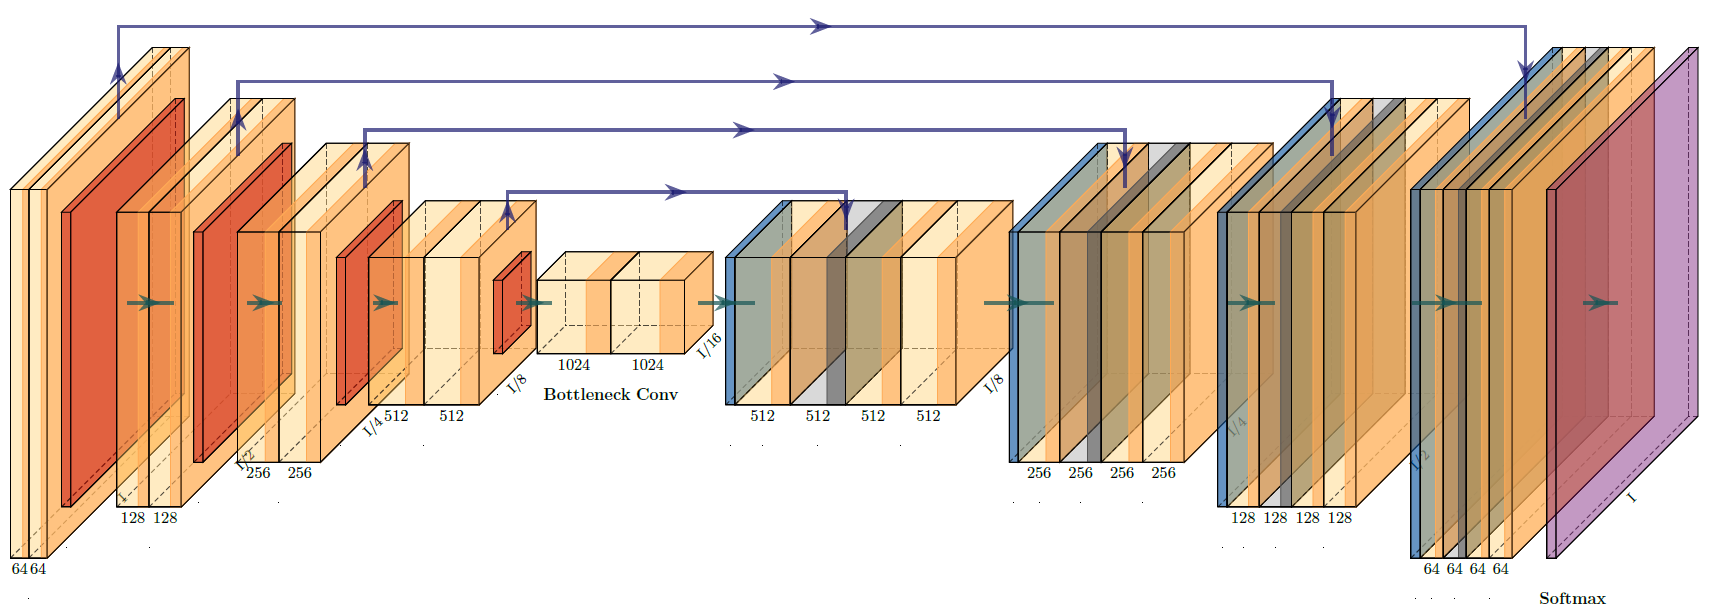
\includegraphics[width=0.85\textwidth]{unet.png}
\caption{U-Net model scheme.
The first part of the structure represents the encoder while the tail of the model is the decoder part.
The model name is given by the numerous shortcut connections which link the encoder layers to the decoder ones: if we contract the long-range connections the global structure acquire a U form.
The figure was generated using the \href{https://github.com/HarisIqbal88/PlotNeuralNet}{PlotNeuralNet} package of H. Iqbal.
}
\label{fig:unet}
\end{figure}
\end{center}


%Because the decoding process loses some of the higher level features the encoder learned, the U-NET has skip connections. That means that the outputs of the encoding layers are passed directly to the decoding layers so that all the important pieces of information can be preserved.

\end{document}
